%-------------------1.1
\section{Auto-resizing equation}
\begin{tabular}{l | c}
\begin{minipage}[m]{0.4\textwidth}
\enum{
\resizebox{.6\textwidth}{!}{$\dot{\rho}=
\dfrac{x^3}{45a^9-23b}$}}{1.1}
\end{minipage}
& \begin{minipage}[m]{0.5\textwidth}
\renewcommand\textminus{\mbox{-}}%<<<<<<<<<<<
\begin{lstlisting}[numberstyle=\zebra{black!5}{blue!15},numbers=left,basicstyle=\footnotesize]{tex}
\begin{equation*}\label{eq1}
\resizebox{.4\textwidth}{!}{ % change .4 to 0.5...
$\dot{\rho}=\dfrac{x^3}{45a^9-23b}$} 
\end{equation*}
    \end{lstlisting}
\end{minipage}
\end{tabular}
 
 

%-------------------1.2



\section{Form for simplest calculation}
\begin{tabular}{l | c}
\begin{minipage}[m]{0.4\textwidth}
\enum{ \newcommand{\sss}[1]{this.getField("#1").value}
\begin{Form}
\noindent%
Fill with number \\ 
\small{\mybox[red]{if it does't work try another PDF viewer}}\\ 

\TextField[name=a]{a:} \\

\TextField[name=b]{b:} \\

\TextField[name=c]{c:} \\

\noindent%
$\sum = $ \TextField[name=AvgStat, calculate={
  event.value = ( 
    \sss{a} +
    \sss{b} +
    \sss{c}) ;
}, readonly, value=0]{} 
\end{Form}}{1.2}
\end{minipage}
& \begin{minipage}[m]{0.5\textwidth}
\renewcommand\textminus{\mbox{-}}%<<<<<<<<<<<
\begin{lstlisting}[numberstyle=\zebra{black!5}{blue!15},numbers=left,basicstyle=\footnotesize]{tex}
\documentclass{article}
\usepackage{hyperref}
\begin{document}
\newcommand{\sss}[1]{this.getField("#1").value}
\begin{Form}
\noindent%
Fill with number\\ 

\TextField[name=a]{a:} \\

\TextField[name=b]{b:} \\

\TextField[name=c]{c:} \\
\noindent%
$\sum = $ \TextField[name=AvgStat, calculate={
  event.value = ( 
    \sss{a} +
    \sss{b} +
    \sss{c}) ;
}, readonly, value=0]{} 
\end{Form}
\end{document}
\end{lstlisting}
\end{minipage}
\end{tabular}


%-------------------1.3
\section{Equation in the form of steps}
\begin{tabular}{l | c}
\begin{minipage}[m]{0.4\textwidth}
\enum{ \resizebox{.4\textwidth}{!}{$  \frac{n_0}{n_1} = q_1 + \dfrac{\makebox[\mywd][l]{$1$}}
  {\makebox[\mywd][l]{$q_2 + \dfrac{\makebox[\mywd][l]{$1$}}
  {\makebox[\mywd][l]{$q_3 + \dfrac{\makebox[\mywd][l]{$1$}}
  {\makebox[\mywd][l]{$q_4 + 
   \raisebox{-6pt}{$\ddots$}
   \raisebox{-12pt}{+$\dfrac{\makebox[\mywd][l]{$1\kern30pt$}}
  {q_{k-1} + \dfrac{1}
  {q_k}}$}$}}$}}$}} $}}{1.3}
\end{minipage}
& \begin{minipage}[m]{0.5\textwidth}
\renewcommand\textminus{\mbox{-}}%<<<<<<<<<<<
\begin{lstlisting}[numberstyle=\zebra{black!5}{blue!15},numbers=left,basicstyle=\footnotesize]{tex}
\documentclass{article}
\usepackage{amsmath}
\def\mywd{35pt}
\begin{document}
\[
  \frac{n_0}{n_1} = q_1 + \dfrac{\makebox[\mywd][l]{$1$}}
  {\makebox[\mywd][l]{$q_2 + \dfrac{\makebox[\mywd][l]{$1$}}
  {\makebox[\mywd][l]{$q_3 + \dfrac{\makebox[\mywd][l]{$1$}}
  {\makebox[\mywd][l]{$q_4 + 
   \raisebox{-6pt}{$\ddots$}
   \raisebox{-12pt}{+$\dfrac{\makebox[\mywd][l]{$1\kern30pt$}}
  {q_{k-1} + \dfrac{1}
  {q_k}}$}$}}$}}$}}
\]
\end{document}
\end{lstlisting}
\end{minipage}
\end{tabular}

%-------------------1.4
\section{One number for multiline equation}
\begin{tabular}{l | c}
\begin{minipage}[m]{0.4\textwidth}
\enum{ \begin{equation}
\begin{aligned}
x_{ij} &= d_{ijk}E_k, \\ 
x_{ij} &= \varsigma_{ijk}H_k,\\ 
x_{ij} &= s_{ijkl}X_{kl},\\ 
x_{ij} &= \xi_{ij}\delta p,\\ 
x_{ij} &= \alpha_{ij}\delta T
\end{aligned}
\end{equation}}{1.4}
\end{minipage}
& \begin{minipage}[m]{0.5\textwidth}
\renewcommand\textminus{\mbox{-}}%<<<<<<<<<<<
\begin{lstlisting}[numberstyle=\zebra{black!5}{blue!15},numbers=left,basicstyle=\footnotesize]{tex}
\documentclass{article}
\usepackage{amsmath}
\begin{document}
\begin{equation}
\begin{aligned}
x_{ij} &= d_{ijk}E_k, \\ 
x_{ij} &= \varsigma_{ijk}H_k,\\ 
x_{ij} &= s_{ijkl}X_{kl},\\ 
x_{ij} &= \xi_{ij}\delta p,\\ 
x_{ij} &= \alpha_{ij}\delta T
\end{aligned}
\end{equation}
\end{document}
\end{lstlisting}
\end{minipage}
\end{tabular}

%-------------------1.5
\section{Matrix in \textbf{standalone} documentclass}
\begin{tabular}{l | c}
\begin{minipage}[m]{0.4\textwidth}
\enum{ \begin{equation*}
\begin{matrix} 
a_{11} & a_{12} & a_{13}  \\
a_{21} & a_{22} & a_{23}  \\
a_{31} & a_{32} & a_{33}  \\
\end{matrix} 
\end{equation*} }{1.5}
\end{minipage}
& \begin{minipage}[m]{0.5\textwidth}
\renewcommand\textminus{\mbox{-}}%<<<<<<<<<<<
\begin{lstlisting}[numberstyle=\zebra{black!5}{blue!15},numbers=left,basicstyle=\footnotesize]{tex}
\documentclass[preview,border={-5cm 0cm -5cm -0.1cm}]{standalone}
\usepackage{amsmath}
\begin{document}
\begin{equation*}
\begin{matrix} 
a_{11} & a_{12} & a_{13}  \\
a_{21} & a_{22} & a_{23}  \\
a_{31} & a_{32} & a_{33}  \\
\end{matrix} 
\end{equation*}
\end{document}
\end{lstlisting}
\end{minipage}
\end{tabular}


%-------------------1.6
\section{Multiple lines, one centered label}
\begin{tabular}{l | c}
\begin{minipage}[m]{0.4\textwidth}
\enum{ \begin{equation} \label{eq1}
\begin{split}
A & = \frac{\pi r^2}{2} \\
 & = \frac{1}{2} \pi r^2
\end{split}
\end{equation} }{1.6}
\end{minipage}
& \begin{minipage}[m]{0.5\textwidth}
\renewcommand\textminus{\mbox{-}}%<<<<<<<<<<<
\begin{lstlisting}[numberstyle=\zebra{black!5}{blue!15},numbers=left,basicstyle=\footnotesize] 
\begin{equation} \label{eq1}
\begin{split}
A & = \frac{\pi r^2}{2} \\
 & = \frac{1}{2} \pi r^2
\end{split}
\end{equation}
\end{lstlisting}
\end{minipage}
\end{tabular}

%-------------------1.7
\section{Array as a fraction}
\begin{tabular}{l | c}
\begin{minipage}[m]{0.4\textwidth}
\enum{ 
$I-IV-V^{\substack{6-4\\4-3\\6-4\\4-3}}-I-cadence$ \\

$I-IV-V^{\genfrac{}{}{0pt}{}{6-4}{4-3}}-I-cadence$ \\

$I-IV-V^{\begin{array}{c}6-4\\4-3\\ \end{array}}-I-cadence$}{1.7}
\end{minipage}
& \begin{minipage}[m]{0.5\textwidth}
\renewcommand\textminus{\mbox{-}}%<<<<<<<<<<<
\begin{lstlisting}[numberstyle=\zebra{black!5}{blue!15},numbers=left,basicstyle=\footnotesize] 
\documentclass{article}
\usepackage{amsmath}

\begin{document}
$I-IV-V^{\substack{6-4\\4-3\\6-4\\4-3}}-I-cadence$ \\

$I-IV-V^{\genfrac{}{}{0pt}{}{6-4}{4-3}}-I-cadence$ \\

$I-IV-V^{\begin{array}{c}6-4\\4-3\\ \end{array}}-I-cadence$
\end{document}
\end{lstlisting}
\end{minipage}
\end{tabular}

%-------------------1.8
\section{Aligning equations inbetween text}
\begin{tabular}{l | c}
\begin{minipage}[m]{0.4\textwidth}
\enum{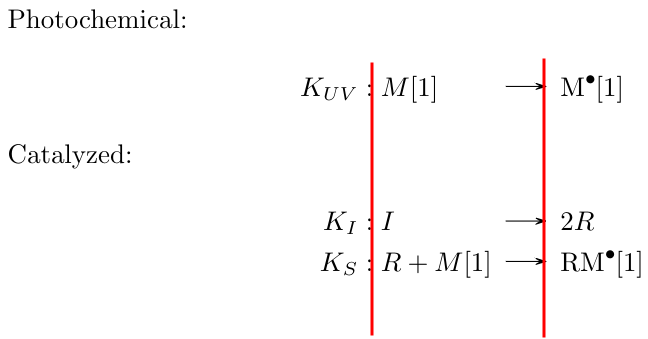
\includegraphics[width=1\linewidth]{1.8.png}}{1.8}
\end{minipage}
& \begin{minipage}[m]{0.5\textwidth}
\renewcommand\textminus{\mbox{-}}%<<<<<<<<<<<
\begin{lstlisting}[numberstyle=\zebra{black!5}{blue!15},numbers=left,basicstyle=\footnotesize] 
\documentclass{article}
\usepackage{amsmath}

\begin{document}
\begin{alignat*}{2}
\intertext{Photochemical:}
K_{UV} &: M[1]& &\ch{-> M^{*}}[1]
\intertext{Catalyzed:}
K_I &: I& &\ch{->} 2R \\
K_S &: R + M [1]& &\ch{-> RM^{*}}[1]
\end{alignat*}
\end{document} 
\end{lstlisting}
\end{minipage}
\end{tabular}

%-------------------1.9
%-------------------1.10
%-------------------1.11
%-------------------1.12
%-------------------1.13
%-------------------1.14


 
